
%\setcounter{chapter}{42}
\chapter{How to Do Research\index{Research}}
\label{chapter:how_to_do_research}

\section{Introduction}

The jump from problem sets into research 
can be hard.  Sometimes we see students who ace their
classes but struggle with their research.  In little bites, here is what we think is important for succeeding in research as a graduate student.  This chapter is written as advice from research advisor to a graduate student (so we use use the first person in the text), but we hope that this advice will be useful for anyone learning how to create and debug research or engineering projects.

\section{Research Advice}

The first piece of advice can go on a bumper sticker: {\bf ``Slow down to speed up.''}   In
  classes, the world is rigged.  There's a simple correct answer and the problem is structured to let you come to that answer.  You get  feedback with the correct answer within a day after you submit  anything.

Research is different.  No one tells you the right answer, and we may not know if there is a right answer.  We don't know if something doesn't work because there's a  silly mistake in the program or because a broad set of assumptions is flawed.

How do you deal with that?  Take things slowly.  Verify your
assumptions.  Understand the thing, whatever it is---the program, the algorithm,  or the
proof.  As you do experiments, only change one thing at a time, so you know what the outcome of the experiment means.

It may feel like you're going slowly, but you'll be making much more progress than if you flail around, trying different things, but not understanding what's going on. \\

\begin{figure}[htpb!]
\centerline{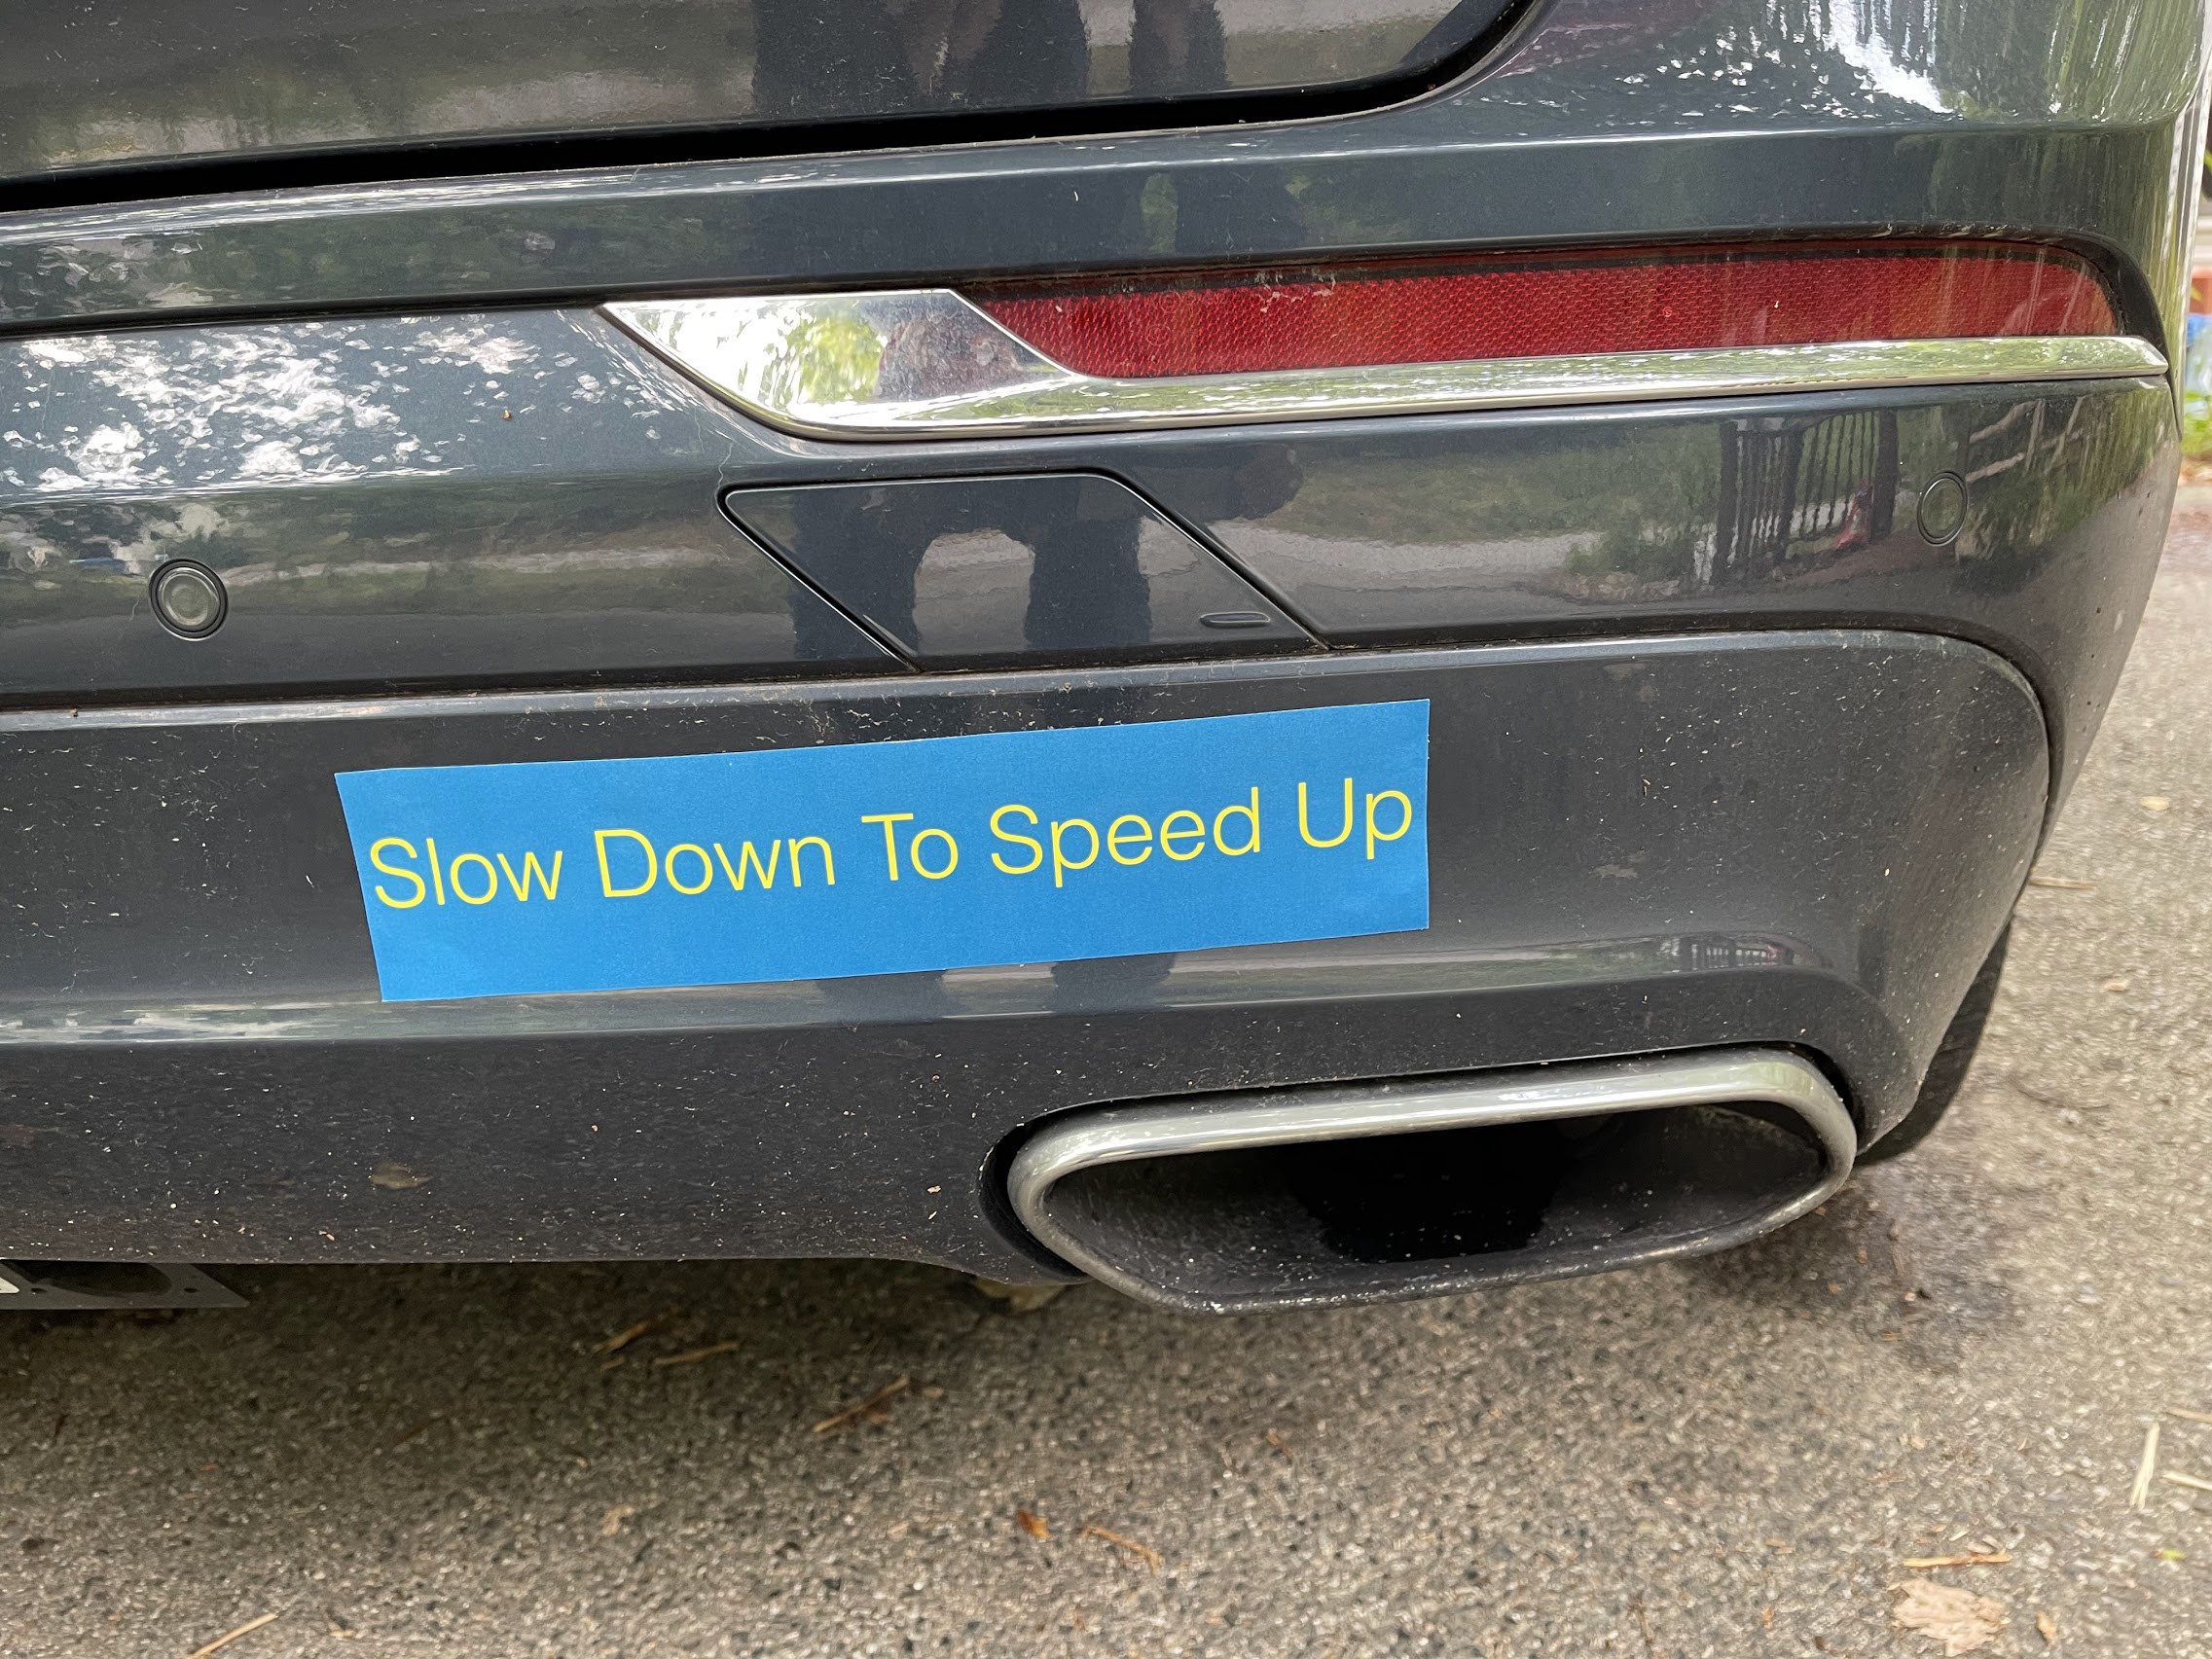
\epsfig{file=figures/how_to_do_research/bumper.jpg,width=2.5in}}
\caption{Research advice for a bumper sticker.}
\label{fig:vw}
\end{figure}


%% http://bethpartin.com/denver-photos-vw-bus-on-capitol-hill/
\noindent {\bf Please don't tell me ``it doesn't work.''}  
  Of course, it doesn't work.  If there's a single mistake in the    chain, the whole thing won't work, and how could you possibly go  through all those steps without making a mistake somewhere?  What I want to   hear instead is something like, ``I've narrowed down the problem to   step B.  Until step A, you can see that it works, because you put in
  X  and you get Y out, as we expect.   You can see how it fails here
  at   B.  I've ruled out W and Z as the cause.'' \\
  
\noindent {\bf ``This sounds like hard work.''}  Yes.  It's no longer about being  smart.  By now, everyone around you is smart.  In graduate school,   it's the {\em  hard workers} who  pull ahead.  This happens  in sports, too.  You always read stories about how hard the great players work, being the first ones out to practice, the last ones to
  leave, and so on. \marginnote{A co-author, who generally works harder than I do, tells me I should add comments here about the importance of taking time off from work and maintaining a good life/work balance.  That is true: you should work at a pace you can sustain, and you should refresh yourself by making time for the things that matter more than work, such as relationships, service, and relaxation.  Perhaps the point is to protect your time so you will have enough time to do the research well.} \\
  
  
  
\noindent {\bf ``How do I get myself to work hard enough to do research
  well?''}  It all plays out if you love what you're doing.
  You become good at it because you spend time at it and you do that because you enjoy it.
  So pick something to work on that you can love.   If
  you're not the type who falls in love with a problem, then just know   that working hard is what you have to do to succeed at research. \\
  
\noindent {\bf The above isn't completely true.}  Beyond
  working hard, there's also {\em steering}.  We're like boats.  We need
  motors---that's the part about working hard.  But we also need a rudder for
  steering---that means stepping back periodically to make sure
  we're working on the right thing.  On the topic of steering,
  I find time management books to be very helpful.  They teach you how  to spend your time solving the right problems. \\
  
\noindent {\bf Toy models.}
There's a concept I want a
  simple phrase for, and maybe you can help me think up a good name.
  It's ``the simplest toy model that captures the main
  idea''  (TSTMTCTMI).    Anyway, simple toy models
 always help me.  With a good one, 
  you can build up intuition about what matters, which is a big
  advantage in research.  

Here's an example.  The color constancy problem is to estimate surface
reflectance colors when we only get to observe the
wavelength-by-wavelength product of the each surface
reflectance spectrum and the unknown
illuminant spectrum.  A toy model for that problem is to try to estimate the scalars
$a$ and $b$ from only observing their product, $y = a \times b$.  There's a
surprising richness even to this simple problem, and thinking about it
allows you to think through loss functions and other aspects of
Bayesian decision theory (\fig{\ref{fig:toy}}).  I co-authored a paper that discusses 
$y = a \times b$ for much of the manuscript \cite{Freeman95a}.
Another toy model is to consider,  as a proxy for complicated shaded surfaces, a
single bump.  You get the idea.
\begin{figure}[h]
\centerline{
\epsfig{file=figures/how_to_do_research/abproblem.eps,width=1.4in}}
\caption{A toy model for the color constancy problem:  $y = a \times b$. The plot shows the possible solutions for $a$ and $b$ when $y=1$.}
\label{fig:toy}
\end{figure}

Having the intuitions from working with toy problems gives you a big advantage in the research, because you can figure out what will work by thinking it through with your toy model. \\

\noindent {\bf Strategies for success.}  Here is a parable, as told by my friend Yair Weiss.  There is a weak
and a strong graduate student.  They are both asked by their advisor
to try a particular approach to solving a research problem.
The weak student does exactly what the advisor has asked.  But the advisor's
solution fails, and the student reports that failure.
The strong student starts doing what the advisor has asked, sees that
it doesn't work, looks around within some epsilon ball
of the original proposal to find what does work, and reports that solution.
\begin{figure}[htpb!]
\centerline{
\epsfig{file=figures/how_to_do_research/twoStudents.pdf,width=2in}}
\caption{The parable of the two students.}
\label{fig:students}
\end{figure}
%% http://www.123rf.com/photo_2851187_the-two-students-with-the-book.html

\noindent {\bf Sometimes it's useful to think that everyone else is completely off-track.}  This
  lets you do things that no one else is doing.  It's
  best not to be too vocal about that.  You can say something like,
  ``Oh, I just thought I'd try out this direction.'' \\
  
\noindent {\bf It's also sometimes useful to remember} that many smart people have
  worked on this and related problems and written their thoughts and results
  down in papers.  Don't be caught flat-footed with a large body of closely
  related literature that you aren't familiar with.  \\
  
\noindent {\bf How a business school might talk about your research}.   You have a brand:  you.  There are many impressions you want to build up about your brand:  that person always does great work, they have good
  ideas, they give great talks, they write wonderful software.
  Promote your brand.  Build up a great reputation for yourself by  consistently behaving in the way you'd like to be thought of.\\
% \begin{figure}[htpb!]
% \centerline{
% 
\epsfig{file=figures/how_to_do_research/applered.eps,width=0.6in}}
% \caption{Nurture your research brand.  }
% \label{fig:brand}
% \end{figure}
%% http://hms-somerset-co.blogspot.com/2012/12/apple-logo.html


\noindent {\bf Cultivate your strengths and play to those strengths.}  Some
  possible strengths include  being broad, being creative, being  a great implementer, or being great at doing theory.  \\
  
\noindent {\bf Please don't report to me and say, ``This instance doesn't work.''}  Why  doesn't it work?  Why should it work?   Is there a simpler case we  can make work?  Do you think it's a general issue that affects all
  problems of this category?  Can you think of what's  not working?  Can you contort things
 to make an example that does work?  At the very least, can you make it fail
 worse, so we understand some aspects of the system?  \\
 
\noindent {\bf Progress.} I love to hear about progress when I meet with students, but  note that  I have a very general notion of
 progress.  Progress can include things like ``I've shown why this doesn't work,'' ``I've
 simplified the task to get it to start working,'' or ``I spent the
 whole time reading because I know I have to understand this before I
 can make any progress.'' \\
 
\noindent {\bf Please don't hide from me.}  Let's talk.  I
  like it when you track me down and insist that we talk, for example,  if I've been traveling. \\
  

\noindent {\bf On collaboration.}  Science is generally a team sport.   What matters in a collaboration is whether the work is insightful,  foundational, or impactful.  It doesn't matter that many people were involved.
It is much better to be one of 10 contributors to a great paper than to be the sole author on an unimportant paper. The relationships formed through collaborations can become friendships that last over your career. \\

\noindent {\bf On authorship.}  What names should be on a paper? Everyone who contributed to the paper.  Contributions can be through experimentation, contributing a seminal idea that the paper builds on, or helping with the writing.  Sometimes an authorship contribution can include trying out a research direction that didn't work. If I'm on the fence about whether someone contributed enough to be an author, I usually ask the person themselves, and go with whichever outcome they prefer. 


\section{Concluding Remarks}  


For a presentation to the visiting admitted MIT computer science graduate students, I
  emailed all MIT Computer Science and Artificial Intelligence Laboratory (CSAIL) researchers and faculty members, asking ``Please send me   what you think is   the most important  quality for success in graduate school.''   I compiled their responses (along with photos of the responders) into slides that are available online:  
\begin{verbatim}
http://people.csail.mit.edu/billf/talks/10minFreeman2013.pdf
\end{verbatim}
I think it's a lot of good advice about research. 


\marginnote{{\bf One final note about doing research.}  We hope you love it.  We  certainly do.  The research community is a community of people who are passionate about what they do, and we welcome you to it!}








